\documentclass[a4paper]{article}
%% Language and font encodings
\usepackage{graphicx, cite, verbatim, color, amsmath, amssymb}
\usepackage{listings}
\usepackage{hyperref}
\usepackage{fancyhdr}
\usepackage{algorithm}
\usepackage{algpseudocodex}

\setlength{\abovecaptionskip}{2pt}
\setlength{\belowcaptionskip}{2pt}

% \usepackage{algcompatible}
\usepackage{subcaption}
\usepackage{bm}
\usepackage[compact]{titlesec}


%\setlength{\headheight}{0in}
\setlength{\headsep}{0.3in}
\setlength{\topmargin}{-0.5in}
\setlength{\textheight}{8.8in}
\setlength{\textwidth}{7in}
\setlength{\oddsidemargin}{-.35in}
\setlength{\evensidemargin}{-.35in}
\setlength{\unitlength}{1in}


% useful shortcuts/macros
\newcommand{\be}{\begin{eqnarray}}
\newcommand{\ee}{\end{eqnarray}}
\newcommand{\ben}{\begin{eqnarray*}}
\newcommand{\een}{\end{eqnarray*}}
\newcommand{\mbf}{\mathbf}
\newcommand{\mbfv}[1]{\vec{\mathbf{#1}}}
\newcommand{\sbf}[1]{\boldsymbol{#1}}
\newcommand{\half}{\frac{1}{2}}
\newcommand{\pp}[2]{\frac{\partial #1}{\partial #2}}
\newcommand{\dd}[2]{\frac{d #1}{d #2}}

% \newcommand{\algmargin}{\the\ALG}
% \makeatother
% \newlength{\whilewidth}
%\settowidth{\whilewidth}{\algorithmicwhile\ }
%\algdef{SE}[parWHILE]{parWhile}{EndparWhile}[1]
%  {\parbox[t]{\dimexpr\linewidth-\algmargin}{%
%     \hangindent\whilewidth\strut\algorithmicwhile\ #1\ \algorithmicdo\strut}}{\algorithmicend\ \algorithmicwhile}%
%\algnewcommand{\State }[1]{\State%
%  \parbox[t]{\dimexpr\linewidth-\algmargin}{\strut #1\strut}}
  
% abstract formatting
\RequirePackage[style]{abstract}
\renewcommand{\abstitlestyle}[1]{}
\renewcommand{\abstracttextfont}{\bfseries\normalsize}
\setlength{\absleftindent}{0in}
\setlength{\absrightindent}{0in}

% caption formatting
\RequirePackage[tableposition=top]{caption}
\captionsetup*{font=bf}

% code listing formatting
\definecolor{commentgreen}{RGB}{14,120,0}
\lstset{
  numbers=none, 
  basicstyle=\scriptsize, 
  commentstyle=\color{commentgreen},
  keywordstyle=\bf\color{blue},
  language=python, 
  frame=shadowbox,
  rulesepcolor=\color{black},
  flexiblecolumns=true,
  extendedchars=false,
  showstringspaces=false,
  keepspaces=true
}

% packed itemize
\newenvironment{itemizePacked}{
\begin{itemize}
  \setlength{\itemsep}{0pt}
  \setlength{\parskip}{0pt}
  \setlength{\parsep}{0pt}
}{\end{itemize}}

% packed enumerate
\newenvironment{enumeratePacked}{
\begin{enumerate}
  \setlength{\itemsep}{-1pt}
  \setlength{\parskip}{0pt}
  \setlength{\parsep}{0pt}
}{\end{enumerate}}


% no indent
\setlength{\parindent}{0pt}

% column separation
\setlength{\columnsep}{3ex}

% header
\fancyhead[L]{
\large \sc
Entropy Stability
}
\renewcommand{\headrulewidth}{1pt}
\pagestyle{fancy}

% section spacing
\titlespacing{\section}{0pt}{12pt}{4pt}
\titlespacing{\subsection}{0pt}{8pt}{2pt}

%section numbering for equations 
\numberwithin{equation}{section}
\makeatletter
\@addtoreset{equation}{section}
\makeatother
\title{AEROSP 590: Entropy Stability}
\author{Andi Zhou}
\begin{document}
\maketitle

\section{Entropy Condition - Origin and Formulation}
In this section we explain the entropy condition, and explain why this would be necessary in solving Hyperbolic Partial Differential Equations. To explain the neccesity of entropy condition, we first start but discussing a typical conservation law.

\begin{equation} \label{singleConservationLaw}
    \partial_t u^j + \partial_x f^j = 0
\end{equation}
where $f$ is a non-linear function of $U$, where:
\begin{equation}
    \frac{df}{du} = a(u)
\end{equation}
Using chain rule, we could write Equation \ref{singleConservationLaw} as:
\begin{equation}\label{singleConservationLaw_wavespeed}
    u_t + a(u)u_x = 0
\end{equation}
If $u$ is constant along a characteristic trajectory, we also know that $a$ will be constant as well. $u$ would propagate along space in speed $a$. Therefore, we also define $a$ as the signal speed. The trajectories of $u$ would be defined as a characteristics. Equation \ref{singleConservationLaw} is known as the strong (differential) form of the PDE, where a solution to this equation would need to satisfy the differential operators at all points in space and time. A solution that matches the strong form is known as the a strong solution. However, the differential form could not admit discontinuities. Consider, for example, the inviscid Burger's equation:
\begin{equation}
    \partial_t u + u \partial_x u = 0
\end{equation}
Where now the wavespeed depends upon the state $a(u) = u$. If we draw the characteristic curve of the Burger's equation subject to a Gaussian initial condition, we would find that the characteristic lines may eventually intersect at one point (Figure \ref{BurgerEquationFigure}). 
\begin{figure}[H]
    \centering
    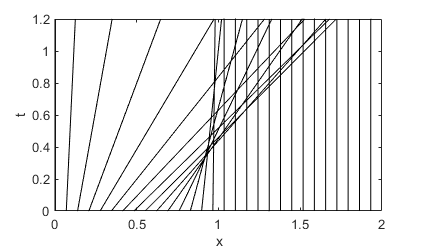
\includegraphics[width=10cm]{fig/BurgersCharacteristic.png}
    \caption{Example characteristic curve of Burger's equation}
    \label{BurgerEquationFigure}
\end{figure}
The above figure is subjected to the following initial condition:
\begin{equation}
    u(x,0) = 
    \begin{cases}
        \sin^2 (\pi x) & 0 \leq x \leq 1 \\
        0 & 1 \leq x \leq 2
    \end{cases}
\end{equation}
We see that due to the difference the state, the slope ($1/a$) varies across the domain which causes characteristic lines to intersect each other. At the point of intersection, then, there exists two states, which represents a discontinuity. This is impossible when considering the strong form (Equation \ref{singleConservationLaw}). Then, we require a different formulation of the above conservation law.
\subsection{The Weak Form of Conservation Law}
We now consider the weak form:

\begin{equation}\label{eq:integralConservationLaw}
    \int_{0}^{\infty} \int_{-\infty}^{\infty} \big[w_t u + w_x f(u) \big] dx dt + \int_{\infty}^\infty w(x,0) \phi(x) dx = 0
\end{equation}
where $w$ is any smooth test function with compact support (non-zero only within the specified element). The general idea of weak solution is that we could rewrite the derivatives of $u$ as derivatives of compact test function $w$. From this, we basically eliminated the need for solution to be continuous. However, for hyperbolic systems (which we are interested in), the notion of weak solution \textbf{does not} guarantee uniqueness. Therefore, we need some sort of criterions to select a solution that is \textit{physical}. We then have the \textbf{entropy} condition. 

In order to better study the region of discontinuity, we turn to Equation \ref{singleConservationLaw} and add a term of dissipation at the end:
\begin{equation} \label{eq:artificial_viscosity}
   u_t + f_x = \epsilon u_{xx}
\end{equation}
The term on the right hand side is also known as artificial viscosity. This allows us to identify relevant solutions as limits of solutions of equations with some dissipation. As $\epsilon \rightarrow 0$, the solution would tend towards Equation \ref{singleConservationLaw} in a \textit{weak} sense. 

Now, we consider a convex function $U(u)$ that is a function $u$ and its corresponding convex flux $F(u)$. We assume that these convex function also satisfy a separate form of conservation law:
\begin{equation}
    U_t + F_x = 0
\end{equation}

Again from [], we understand that if the convex function $U$ satisfies a conservation law then multiplying the system by $U_j$, would put the system into \textit{symmetric hyperbolic form}.

We use the above theorem, and we multiply Equation \ref{eq:artificial_viscosity} by $U_j$, and we arrive at the following:
\begin{equation}
    \partial_t U + \partial_x F = \epsilon \sum U_j u^j_{xx}
\end{equation}

Lax introduced the following identity:
\begin{equation}
    \partial_x^2 U = \sum U_j \partial_x^2 u^j + \sum U_{jk} \partial_x u^j \partial_x u^k
\end{equation}
From above, we could deduce that:
\begin{equation}
    \partial_x^2 U \geq \sum U_j \partial_x^2 u^j
\end{equation}
Since we know that $\epsilon > 0$ in Equation \ref{eq:artificial_viscosity}, we could use the above equation estimate the right side:
\begin{equation}
    \partial_t U + \partial_x F \leq \epsilon \partial_x^2 F
\end{equation}
Take $\epsilon \rightarrow 0$, we then recover the entropy condition:
\begin{equation}
    \partial_t U + \partial_x F \leq 0
\end{equation}

We note that, if $u$ is a piecewise continous solution to Equation \ref{singleConservationLaw}, we could arrive at the following assuming we are at a point of discontinuity:
\begin{equation}
    s \big[U\big] - \big[F\big] \leq 0
\end{equation}
where $s$ is the speed of the discontinuity while $\big[\cdot\big]$ denotes jump in the respective quantity across the discontinuity. The above relation is analogous to the Rankine-Hugoniot jump relation:
\begin{equation}
    s \big[u^j\big] - \big[f^j\big] = 0
\end{equation}
We could actually rewrite the entropy condition as follow:
\begin{equation}
    \frac{f(u) - f(u_L)}{u-u_L} \geq S \geq \frac{f(u) - f(u_R)}{u-u_R}
\end{equation}
This is known by Oleinik[] as \textit{Condition E}. If we use the Rankine-Hugoniot jump relation:
\begin{equation}
    f(u_R) - f(u_L) = S(u_R - u_L)
\end{equation}
we also arrive at the \textit{Lax entropy condition} []:
\begin{equation}
    a(u_l) > S > a(u_r)
\end{equation}
%%Commented it out just cuz
\begin{comment}
It is rather difficult to trace when the notion of entropy condition was first introduced. Earliest written work that could be traced on this subjects were done by P. Lax [citation] and O. Oleinik [citation]. Both authors have mentioned the idea of \textit{entropy conditions} repeatedly in their text. 
\end{comment}


%----------------------------------------
\section{Entropy Satisfied Schemes}
Several fluxes satisfy the above entropy condition. We understood from Lax [] that any monotone scheme satisfy the entropy condition. In this section we specifically focus on first order scheme, and list two of these fluxes below.

\subsection{Lax-Friedrich's Scheme}
The Lax-Friedrich scheme, under a specific CFL number, satisfies the entropy condition. The scheme is introduced by Lax in 1954 as a method of discretizing the first order hyperbolic equation without violating the entropy condition introduced in the above section. We introduce the general scheme below, and demonstrate that it is actually a FTCS (forward in time, centered in space) scheme with the temporal derivative replaced by a spatial average of the neighboring points. 
The general Lax-Friedrich discretization is as follow:
\begin{equation}
    \begin{split}
        u_t &= \frac{1}{\Delta t}\big( u^{n+1}_j - \frac{u^n_{j-1} + u^n_{j+1}}{2} \big)  \\
        f_x &= \frac{1}{2\Delta x}\big(f(u^n_{j+1}) - f(u^n_{j-1})\big)
    \end{split}
\end{equation}
Combined together, we obtain the Lax-Friedrich scheme:
\begin{equation}
    \begin{split}
        &\frac{1}{\Delta t}\big( u^{n+1}_j - \frac{u^n_{j-1} + u^n_{j+1}}{2} \big) + \frac{1}{2\Delta x}\big(f(u^n_{j+1}) - f(u^n_{j-1})\big) = 0 \\
        &u_j^{n+1} = \frac{1}{2}(u_{i+1}^n + u_{i-1}^n) - \frac{\Delta t}{2\Delta x}\big(f(u^n_{j+1}) - f(u^n_{j-1})\big)
    \end{split}
\end{equation}
We note that the above scheme is essentialy FTCS:
\begin{equation}
    u_j^{n+1} = \underbrace{\frac{1}{2}(u_{i+1}^n + u_{i-1}^n)}_{\text{Temporal Derivative}} - \underbrace{\frac{\Delta t}{2\Delta x}\big(f(u^n_{j+1}) - f(u^n_{j-1})\big)}_{\text{Spatial derivative (Centered in Space)}}
\end{equation}
According to Lax[], the Lax-Friedrich scheme satisfies the entropy condition under a suitable choice of the $\lambda = \frac{\Delta t}{\Delta x}$.

The Lax-Friedrich scheme satisfies the entropy condition as long as the $\lambda = \frac{\Delta t}{\Delta x}$ satisfies the following criterion:
\begin{equation}
    c\lambda \leq \sqrt{1+m/M-1}
\end{equation}
where $M$ and $m$ are the minimum and maximum eigenvalues of the entropy function Jacobian $\frac{\partial^2}{\partial^2 u}U$ and $c$ denotes the norm of the entropy function derivative $\frac{\partial}{\partial u} U$. The complete proof is presented in section 1 of []. The above inequality could also be transformed in terms of the Courant-Friedrich-Lewy (CFL) number, where the scheme is entropy stable if:
\begin{equation}
    CFL = \frac{a \Delta t}{\Delta x} \leq 1
\end{equation}
where for a $CFL \leq 1$, the Lax-Friedrich scheme is monotone, which satisfies the entropy condition according to Lax [].


%---------------------------------------------------------
\subsection{Engquist-Osher Scheme}
The E-O scheme, or Engquist and Osher scheme could be considered as a modified version of the Cole-Murman scheme used for small disturbance equation of transonic flow.  Engquist and Osher introduced this scheme in a paper publised in 1980 [] and then later generalized this scheme for general hyperbolic systems of conservation laws []. We discuss the formulation of this particular scheme here along with its relevant mathematical proofs.
Consider a non-linear scalar conservation law in 1D:
\begin{equation} 
    w_t + f(w)_x = 0,\\ w(x,t=0) = \Phi(x). \ =\infty < x< \infty
\end{equation}
The solution is approximated by a mesh function $w_j^n$ on the mesh ${(x_J,t^n)}$ with $x_j = k \Delta x, t^n = n \Delta t, j = 0, \pm 1,...,n=0,1,...$. In explicit form, the finite difference approximation is defined as:
\begin{enumerate}
    \item 
\begin{equation} \label{eq:E-O Conservation Law}
    \begin{split}
        w_j^{n+1} &= w_j^n - \frac{\Delta t}{\Delta x}\big(\Delta_{+} f_{-} (w_j^n) + \Delta_{-} f_{+} (w_j^n) \big) \\
        w_j^0 &= \Phi(x_j), j = 0, \pm 1, \pm 2\\
    \end{split}
\end{equation}
    \item \label{eq:E-O_CFL}
        \begin{equation}
            \frac{\Delta t}{\Delta x} \text{sup} |f'| < 1
        \end{equation}

\end{enumerate}
We denote here as a reminder that Part 1 is the fully-discrete version of Equation \ref{eq:E-O Conservation Law} written is a per cell. We specify here as well the following notations:
\begin{equation}
    \begin{split}
        \Delta_{\pm} w_j &= \pm (w_{j\pm 1} - w_j)\\
        D_{\pm} w_j &= \frac{1}{\Delta x} \Delta_{\pm} w_j\\
    \end{split} 
\end{equation}
The auxiliary functions $f_+$ and $f_-$ are:
\begin{equation}
    \begin{split}
        f_+ (w) &= \int_0^w \mathcal{X} (w) f'(w) dw\\
        f_- (w) &= \int_0^w (1 - \mathcal{X}(w)) f'(w)dw\\
    \end{split}
\end{equation}
When $f$ is convex, the definitions then reduce to:
\begin{equation}
    \begin{split}
        f_+ (w) &= f(\mathrm{max}(w,\bar{w}))\\
        f_- (w) &= f(\mathrm{min}(w,\bar{w})) \\
    \end{split}
\end{equation}

where $\bar{u}$ is the stagnation or sonic point for which $f'(\bar{u}) = 0$. We make a note that when the sign is positive, Equation \ref{eq:E-O Conservation Law} becomes the \textit{upwind} algorithm. This is also known as \textit{flux decomposition}, where we separated the original upwinding flux into essentially a decreasing and increasing components. Decomposing this flux into different components provides us with a different perspective when looking at states near shock points.

When we consider a hyperbolic PDE with convex flux, we arrive at the following:
\begin{equation}
    \begin{split}
        f^+ (w) &= 
        \begin{cases}
            f(w), & w \geq \bar{w}\\
            f(\bar{w}), & w \leq \bar{w}\\
        \end{cases}\\
        f^-(w) &= 
        \begin{cases}
            f(w), & w \leq \bar{w} \\
            f(\bar{w}), & w \geq \bar{w}\\
        \end{cases}\\
    \end{split}
\end{equation}
If we have Burger's equation, then the flux becomes: $f(u) = \frac{u^2}{2}$:

\begin{equation}
    \begin{split}
        f^+ (u) &= 
        \begin{cases}
            \frac{u^2}{2}, & u \geq u^*\\
            0, & u \leq u^*\\
        \end{cases}\\
        f^-(u) &= 
        \begin{cases}
            \frac{u^2}{2}, & u \leq u^* \\
            0, & u \geq u^*\\
        \end{cases}\\
    \end{split}
\end{equation}
If we consider an arbitrary, following the notation from Equation \ref{eq:E-O Conservation Law}, we have, 
\begin{equation}
    \Delta_- f_+ = f^+(w_j) + f^-({w_{j+1}})
\end{equation}
The Engquist and Osher scheme demonstrated computational advantages over all previous schemes including Godunov's and Cole-Murman, especially for implicit calculations where a much large time steps could be taken for E-O. It also elimnates the non-physical expansion shocks (satisfies the entropy condition) that plagues the C-M and Roe's method, and also possesses \textit{smoother} flux functions than that of Godunov's.

The E-O scheme is \textit{monotone} if the CFL condition (Equation \ref{eq:E-O_CFL}) is valid[]. Lax proved in [] that monotone schemes always satisfy the entropy condition and converge to a physically relevant solution. From this theorem, we then know that E-O scheme is entropy stable if the CFL condition if Equation \ref{eq:E-O_CFL} is satisfied.

%----------------------------------------------------------------------
\section{The Roe Scheme and Roe's Average}
Philip Roe first introduced the Roe scheme in 1980 in his paper \textit{Approximate Riemann Solvers, Parameter Vectors, and Difference Scheme} []. In his paper, Roe argued that an exact solution to the Riemann problem may not be necessary and we could construct an \textit{approximate} solutions which are the \textit{exact} solutions to an approximate, \textit{linearized} Riemann problem. This section talk mainly on the Motivation and derivation of the Roe scheme. Section \ref{sec:RoeFluxAlgorithm} provides details on the implementations of Roe flux. 
\subsection{Motivation}
Consider again the one-dimensional linear advection equation:
\begin{equation}
    u_t + a(u)u_x = 0
\end{equation}
where $a(u)$ is typically a non-linear. Instead, we construct a linearized problem defined locally at each cell interface:
\begin{equation}
    \mathbf{u}_t + \tilde{A}\mathbf{u}_x = 0
\end{equation}
where $\tilde{A}$ is to be chosen such that it satisfies the \textit{local} conditions, i.e based on $A_L$ and $A_R$. The intuitive candidates are, of course:
\begin{equation}
    \begin{split}
        \tilde{A} &= \frac{1}{2}(A_L + A_R)\\
        \tilde{A} &= A(\frac{1}{2}(\mathbf{u}_L + \mathbf{u}_R))\\
    \end{split}
\end{equation}
However, Roe listed out the following properties that the matrix $\tilde{A}$ has to satisfy:
\begin{enumerate}
    \item Linear mapping from the vector space $\mathbf{u}$ to the vector space $\mathbf{F}$
    \item As $\mathbf{u}_L \rightarrow \mathbf{u}_R \rightarrow \mathbf{u}, \tilde{A}(\mathbf{u}_L,\mathbf{u}_R) \rightarrow A(\mathbf{u})$ where $A = \frac{\partial \mathbf.
    F}{\partial \mathbf{u}}$. In words, the approximate Jacobian $\tilde{A}$ must match with the exact Jacobian $A$ as $\mathbf{u}_L$ and $\mathbf{u}_R$ approaches $\mathbf{u}$
    \item For any $\mathbf{u}_L, \mathbf{u}_R, \tilde{A}(\mathbf{u}_L, \mathbf{u}_R)\times (\mathbf{u}_L - \mathbf{u}_R) = \mathbf{F}_L - \mathbf{F}_R$. In words, conservation must be satisfied.
    \item The eignvectors of $\tilde{A}$ are linearly independent, which means thats the PDE has to be \textit{hyperbolic}.

\end{enumerate}
The above conditions are named Property U, as they are intended to possess uniform validity across discontinuities. In addition, matrix $\tilde{A}$ is sometimes called \textit{Roes's matrix}. It is to be noted that none of the suggestions for $\tilde{A}$ above satisfies the third property. 

We then follow that the matrix $\tilde{A}$ could be constructed from mean value theorems which would arrive at the following:
\begin{equation}
    \tilde{A} = \int_0^1 A(\theta) d \theta
\end{equation}
where $\theta$ is a parameter that vary linearly between 0 and 1 along a straight path connecting each state. However, there is no guarantee that there would exist a candidate that satisfies the integral along with the above listed condition. In addition, it is generally not possible to evaluate the above integral within a closed form for most nonlinear problems of interest.

Roe made a significant breakthrough in his paper by a \textit{change of variable}, that made the integral much easier to evaluate. We will demonstrate in the next section for Euler's equation how this change of parameter led to the Roe's average. Generally, the new parameter should be chosen such that the original states could be expressed as a polynomial for ease of taking derivatives and integration.

\subsection{Roe's Average and  Euler's Equation}
Roe introduced the following parameter vector:
\begin{equation}
    \mathbf{w} = \sqrt{\rho} 
    \begin{bmatrix}
        1\\
        u\\
        v\\
        w\\
        H\\
    \end{bmatrix}
\end{equation}
we notice that via this construction, the original states and fluxes are expressed as a quadratic combination of $\mathrm{w}_i$, i.e $u_1 = \mathrm{w}_1^2$ and $f_1 = \mathrm{w}_1 \mathrm{w}_2$. We then proceed to express the jump in $\mathbf{u}$ and $\mathbf{F}$ in terms of jump in the parameter vector $\mathbf{w}$.

\begin{equation}
    \begin{split}
        \big(\mathbf{u}_L - \mathbf{u}_R\big) &= \tilde{B}(\mathbf{w}_L - \mathbf{w}_R)\\
        \big(\mathbf{F}_L - \mathbf{F}_R\big) &= \tilde{C}(\mathbf{w}_L - \mathbf{w}_R)\\
    \end{split}
\end{equation}
where the first equation provides a link for $\mathbf{w}$ in terms of $\mathbf{u}$. We are looking for matrix $\tilde{B}$ and $\tilde{C}$, which Roe gave in [] as follow:
\begin{equation}
    \begin{split}
        \tilde{B} &=
        \begin{pmatrix}
            2 \bar{\mathrm{w}}_1 & 0 & 0 & 0 & 0\\
            \bar{\mathrm{w}}_2 & \bar{\mathrm{w}}_1 & 0 & 0 & 0\\
            \bar{\mathrm{w}}_3 & 0 & \bar{\mathrm{w}}_1 & 0 & 0\\
            \bar{\mathrm{w}}_4 & 0 & 0 &\bar{\mathrm{w}}_1 & 0 \\
           \frac{\bar{\mathrm{w}}_5}{\gamma} & \frac{\gamma - 1}{\gamma}\bar{\mathrm{w}}_2 & \frac{\gamma - 1}{\gamma }\bar{\mathrm{w}}_3 & \frac{\gamma - 1}{\gamma} \bar{\mathrm{w}}_4 & \frac{\bar{\mathrm{w}}_1}{\gamma}
        \end{pmatrix} \\
        \tilde{C} &= 
        \begin{pmatrix}
            \bar{\mathrm{w}}_2 & \bar{\mathrm{w}}_1 & 0 & 0 & 0\\
            \frac{\gamma - 1}{\gamma}\bar{\mathrm{w}}_5 & \frac{\gamma - 1}{\gamma}\bar{\mathrm{w}}_2 & -\frac{\gamma - 1}{\gamma}\bar{\mathrm{w}}_3 & -\frac{\gamma - 1}{\gamma} \bar{\mathrm{w}}_4 & \frac{\gamma - 1}{\gamma} \bar{\mathrm{w}}_1\\
            0 & \bar{\mathrm{w}}_3 & \bar{\mathrm{w}}_2 & 0 & 0\\
            0 & \bar{\mathrm{w}}_4 & 0 & \bar{\mathrm{w}}_2 & 0\\
            0 & \bar{\mathrm{w}}_5 & 0 & 0 & \bar{\mathrm{w}}_2\\
        \end{pmatrix}
    \end{split}
\end{equation}
The $\bar{\cdot}$ indicates the arithmatic average of the selected quanitites. We then obtain $\tilde{A}$ via:
\begin{equation}
    \tilde{A} = \tilde{C}\tilde{B}^{-1}
\end{equation}
From which, Roe then adopted a simplifying convention from the resulting $\tilde{A}$ matrix by dividing through with $\mathrm{w}$:
\begin{equation}
    u = \frac{\bar{\mathrm{w}}_2}{\bar{\mathrm{w}}_1}, \ v = \frac{\bar{\mathrm{w}}_3}{\bar{\mathrm{w}}_1}, \ w = \frac{\bar{\mathrm{w}}_4}{\bar{\mathrm{w}}_1}, \ H = \frac{\bar{\mathrm{w}}_5}{\bar{\mathrm{w}}_1}
\end{equation}
When expanded out (for $u$), it leads to:
\begin{equation}
    u = \frac{\bar{\mathrm{w}}_2}{\bar{\mathrm{w}}_1} = \frac{\rho^{1/2}_L u_L + \rho^{1/2}_R u_R}{\rho_L^{1/2} + \rho_R^{1/2}}
\end{equation}

The above relations are known as the \textit{Roe average}, in which Roe derived when obtaining a suitable $\tilde{A}$ matrix solvinf the linearized Riemann problem. Roe average states are an intermediate state between the two discontinuities and is important because it is the \textit{only} type of averaging that would gaurantee an exact projection of the state jump onto the right eigenvectors. It is to be noted that $\tilde{A}$ is equal to the original matrix $A$ when evaluated with the Roe averaged states above.
%%-----------------------------------------------------------------------------------
\section{Tadmor's Entropy Stability Criterion}
Eitan Tadmor, in his paper written in 1987, introduced a new, general, criterion capable of evaluating entropy conservation of different numerical fluxes. This section summarizes his paper and the two main theorems that he proposed:
\begin{enumerate}
    \item Entropy conservation by means of comparison
    \item Three-point conservative schemes are entropy stable if and only if they contain \textit{more} viscosity than their entropy conservative equivalent
\end{enumerate}
We focus on the derivation and discussion for the first theorem and briefly states the second.

%%-----------------------------------------------------------------------------------
\subsection{Tadmor's Entropy Stability Criterion}
We again consider a one-dimensional conservation law:
\begin{equation}
    \frac{\partial}{\partial t} \mathbf{u} + \frac{\partial}{\partial x}\big[\mathbf{f(u)}\big] = 0
\end{equation}
and we introduce the entropy function $U(u)$, a \textit{convex} function of $u$ along with the entropy flux $F(u)$, which is also a convex function of $u$. We recall the entropy condition:
\begin{equation}\label{eq:EntrpyInequality}
    \frac{\partial V}{\partial t} + \frac{\partial G}{\partial x} \leq 0
\end{equation}
where:
\begin{equation}
    V(\mathbf{v}) = U(\mathbf{u(v)}), \ G(\mathbf{v}) = F(\mathbf{u(v)})
\end{equation}
We also introduce the entropy variable:
\begin{equation}
    \mathbf{v} = \mathbf{v(u)} = \frac{\partial \mathbf
    U}{\partial \mathbf{u}}(\mathbf{u})
\end{equation}
which is one-to-one mapping to $\mathbf{u}(\mathbf{v})$ due to the convexity of $U$. We could then write the conservation equation as follow:
\begin{equation} \label{eq:EntopyConservationEquation}
    \frac{\partial}{\partial t}\big[\mathbf
    u(\mathbf
    v)\big] + \frac{\partial}{\partial x}\big[\mathbf
    g(\mathbf
    v)\big] = 0, \ \mathbf{g(v)} = \mathbf{f}(\mathbf{u}(\mathbf{
    v}))
\end{equation}
We discretize Equation \ref{eq:EntopyConservationEquation} and \ref{eq:EntrpyInequality} and have the following:
\begin{equation} \label{eq:EntropySystem}
    \begin{split}
        &\frac{d}{dt} \big[\mathbf{u}(\mathbf{v_v}(t))\big] = -\frac{1}{\Delta x}\big[\mathbf
        {g}_{\nu+1/2} - \mathbf{g}_{\nu-1/2}\big]\\
        &\frac{d}{dt} V(\mathbf{v_\nu}(t)) + \frac{1}{\Delta x}\big[G_{\nu + 1/2} - G_{\nu - 1/2}\big] \leq 0 \\
    \end{split}
\end{equation}
which are the conservation equation along with its respective entropy inequality. Our end goal is \textit{entropy conservative} schemes, in which only the eqiality hold in Equation \ref{eq:EntrpyInequality}. We multply the first equation of Equation \ref{eq:EntropySystem} by the entropy variable by $\mathbf{v}_\nu^T(t) = U_\mathbf{u}^T(\mathbf{u_\nu(t)})$, which we obtain the following:
\begin{equation}\label{eq:Convert1}
    \frac{d}{dt}V(\mathbf{v}_\nu(t)) = \frac{d}{dt} U(\mathbf{u}_\nu(t)) = -\frac{1}{\Delta x} \mathbf{v}_\nu^T \big[\mathbf{g}_{\nu + 1/2} - \mathbf{g}_{\nu - 1/2}\big]
\end{equation}
which we could subsitute into the entropy condition and have the following equality. The expression:
\begin{equation}\label{eq:Convert2}
    \mathbf{v}_\nu^T \big[\mathbf{g}_{\nu + 1/2} - \mathbf{g}_{\nu - 1/2} \big] = \mathbf{G}_{\nu + 1/2} - \mathbf{G}_{\nu - 1/2}
\end{equation}
is conservative if and only if:
\begin{equation}\label{eq:Tadmor'sEntropyCriteria}
    \Delta \mathbf{v}_{\nu + 1/2}^T \mathbf{g}_{\nu + 1/2} = \Psi_{\nu + 1} - \Psi_\nu, \ \Delta \mathbf{v}_{\nu + 1/2} = \mathbf{v_{\nu + 1}} - \mathbf{v}_\mathbf{\nu}
\end{equation}
This is Tadmor's entropy stability criterion. $\mathbf{g}_{\nu + 1/2}$ could be taken as any numerical flux, while for Euler's equation in 1D:
\begin{equation}
    \begin{split}
        \mathbf{v} &= 
        \begin{pmatrix}
            \frac{\gamma - S}{\gamma - 1}-\frac{\rho u^2}{2p} \\
            \frac{m}{p}\\
            -\frac{\rho}{p}
        \end{pmatrix}\\
        \Psi &= \rho u
    \end{split}
\end{equation} 
Tadmor's new criterion is different in that the amount of numerical viscosity present is essentially \textit{quanitified} and is then later used for Entropy stability evaluation. In addition, it is to be noted that Tadmor's criterion is extremely general, which means that it could be applied to any numerical flux. Any flux could be tested for its entropy conservation by directly substituting the relevant variables and fluxes into Equation \ref{eq:Tadmor'sEntropyCriteria}.


%---------------------------------------------------------------------------------
\subsection{Tadmor's Second Theorem}
In [], Tadmor only proved entropy conservation (i.e Entropy is equal across a cell interface), not stability. He later extended his idea to essentially three-point scheme and proved that: \textit{A conservative scheme which contains more numerical viscosity than that present in the entropy conservative one is entropy stable}. 

Essentially, we consider three points schemes that could be written in the following viscosity form:
\begin{equation} \label{eq:EntropyConservedScheme_Viscosity_form}
    \frac{d}{dt}\big[\mathbf(
    u(\mathbf{v_\nu}(t)))\big] = - \frac{1}{2\Delta x} \big[\mathbf
    {g}(\mathbf{v_{\nu+1}}) - \mathbf{g}(\mathbf{v_{\nu-1}})\big] + \frac{1}{2\Delta x} \big[Q_{\nu + 1/2} \Delta \mathbf{v}_{\nu+1/2} - Q_{\nu + 1/2} \Delta \mathbf{v}_{\mathbf{v}-1/2}\big]
\end{equation}
Where $Q_{\mathbf{v}+1/2}$ is referred to as the numerical viscosity coefficient matrix. We note that the class of three-point schemes includes second-prder accurate TVD schemes such as the High-Resolution Osher flux and a number of other schemes [][]. We then introduce a new variable:
\begin{equation}
    D_{\nu + 1/2} = Q_{\nu + 1/2} - Q_{\nu + 1/2}^*
\end{equation}
which denote the deviation of its viscosity from that of the entropy conservative scheme, which we then have:
\begin{equation}
    \frac{d}{dt}\big[\mathbf(
    u(\mathbf{v_\nu}(t)))\big] = - \frac{1}{2\Delta x} \big[\mathbf
    {g}(\mathbf{v_{\nu+1}}) - \mathbf{g}(\mathbf{v_{\nu-1}})\big] + \frac{1}{2\Delta x} \big[D_{\nu + 1/2} \Delta \mathbf{v}_{\nu+1/2} - D_{\nu + 1/2} \Delta \mathbf{v}_{\mathbf{v}-1/2}\big]
\end{equation}
We could also rewrite the above equation in the form of entropy condition (as per last section), following essentially the same step as outlined in Equation \ref{eq:Convert1} and Equation \ref{eq:Convert2} and use identities outlined in [] to obtain the following:
\begin{equation}
    \begin{split}
        \frac{d}{dt} V(\mathbf{v}_\nu(t)) + \frac{1}{\Delta x}\big[G_{\nu + 1/2} - G_{\nu - 1/2}\big] = -\frac{1}{4\Delta x} \big[\Delta \mathbf{v}_{\nu+1/2}^T D_{\nu + 1/2} \Delta \mathbf{v}_{\nu+1/2} - \Delta \mathbf{v}_{\nu-1/2}^T D_{\nu - 1/2} \Delta \mathbf{v}_{\nu-1/2}\big]
    \end{split}
\end{equation}
We observe that if the scheme is considered to contain more viscosity, then $D$ would be positive, and the overall right hand side of the above equation remains \textit{negative}, which then leads to the entropy condition being satisfied (Equation \ref{eq:EntropySystem}). This theorem allows us to tune additional numerical viscosity such that both entropy stability and second order accuracy could be obtained.

\section{Roe's Entropy Conservative Flux}
In 2006, building on top of Tadmor's theorems presented above, Roe made key contribution in Entropy stable fluxes [] by presenting an \textit{entropy conservative} flux that could be made \textit{stable} via upwinding. In this section, we summarize Roe's contribution and discuss his findings.

\subsection{Entropy Production}
From Tadmor, we know that entropy production across an interface could be characterized by the following equation:
\begin{equation}
    \Delta \mathbf{v}_{\nu + 1/2}^T \mathbf{g}_{\nu + 1/2} - (\Psi_{\nu + 1} - \Psi_\nu), \ \Delta \mathbf{v}_{\nu + 1/2} = \mathbf{v_{\nu + 1}} - \mathbf{v}_\mathbf{\nu}
\end{equation}
where $\mathbf{v}$ represents the entropy variable and $\Psi$ is an arbitrary grid function. For Euler's equation in 1D, the above two quanitites are:
\begin{equation}
    \begin{split}
        \mathbf{v} &= 
        \begin{pmatrix}
            \frac{\gamma - S}{\gamma - 1}-\frac{\rho u^2}{2p} \\
            \frac{m}{p}\\
            -\frac{\rho}{p}
        \end{pmatrix}\\
        \Psi &= \rho u
    \end{split}
\end{equation} 
We use the following short hand $\big[\cdot \big]$ to represent the difference between two neighboring cells. We then have the following entropy production
\begin{equation}
    \big[\mathbf{v}\big] \cdot \mathbf{g} - \big[\Psi\big]
\end{equation}
It could be shown that if the flux is of central difference type $g = \bar{g}$, then the entropy production is of 3rd order:
\begin{equation}
    \big[\mathbf{v}\big] \cdot \bar{g} = \mathcal{O}(\delta^3)
\end{equation}
The third order production is small in smooth region, large across shocks and incorrect across rarefraction waves. The large production production across shocks are essentially correct since entropy across shocks should increase. However, it is incorrect across rarefractions as entropy production should be zero across rarefraction waves. We at first seek to construct an entropy conservative flux, which for Euler's equations, satisfy the following:
\begin{equation}
    \big[\mathbf{v}\big] \cdot \mathbf{g} = \big[\rho u\big]
\end{equation}
Roe then introduced the following Entropy conservative flux:


\subsection{An Entropy Conservative Flux}
Similar to the Roe flux derivation, we at first define a parameter vector for change of variable:
\begin{equation}
    \mathbf{z} = \sqrt{\frac{\rho}{p}} (1, u, p)
\end{equation}
from which we could redefine our state vector (For Euler's Equation) as:
\begin{equation}
    \mathbf{u}(\mathbf{z}) = 
    \begin{bmatrix}
        \rho\\
        \rho u \\
        E\\
    \end{bmatrix} = 
    \begin{bmatrix}
        z_1 z_3\\
        z_2 z_3\\
        \frac{1}{\gamma - 1} \frac{z_3}{z_1} + \frac{1}{2} \Bigl(\frac
        {(z_2z_3)^2}{z_1z_3} \Bigr)
    \end{bmatrix}
\end{equation}
which we could then redefine the entropy variable as:
\begin{equation}
    \mathbf{v} = \big(\frac{\gamma}{\gamma - 1} + \frac{\gamma + 1}{\gamma -1} \ln z_1 + \ln z_3 - \frac{1}{2} z_2^2, z_1 z_2, -z_1^2\big)^T
\end{equation}
Tadmor in 2003 arrived at an explicit solution for an entropy conservative flux:
\begin{equation}
    f^* = \sum_k \frac{\big[ \rho u\big]_{k + \frac{1}{2}}}{ \big[ \mathbf{v}\big] \cdot \delta \mathbf{u}_{k + \frac{1}{2}}} \delta \mathbf{u}_{k+1/2}
\end{equation}


We then have the following flux:
\begin{equation}
    \begin{split}
        f_1^* &= \bar{z}_1 \bar{z}_3^{\ln}\\
        f_2^* &= \frac{\bar{z}_3 + \bar{z}_2 f_1^*}{\bar{z}_1}\\
        f_3^* &= \frac{1}{2\bar{z}_1}\big(\frac{\gamma + 1}{\gamma -1} \frac{f_1^*}{z_1^{\ln}} + \bar{z}_2 f_2^* \big)
    \end{split}
\end{equation}
This flux exactly preserves entropy across discontinuities. In addition, note that logarithmic mean, $(\cdot)^{\ln}$, is used here. 
logarithmic mean is defined as follow:
\begin{equation}
    L(x_1,x_2) = \frac{x_1 - x_2}{\ln x_1 - \ln x_2}
\end{equation}
We see that if $x_1$ and $x_2$ both approach $x$, then the entire expression would reduce to $x$. This average allows us to replace $\big[\ln p\big]$ with $\frac{\big[p\big]}{p^{\ln}}$ where $p^{\ln} = L(p_L,p_R)$.
Another reason why logarithmic mean maybe preferred more than arithmatic mean is their tendency to take a lower mean of when the pair of number givens are extremely far apart. Therefore this will act as an limiter that limits the flux states when encoutering disconnected values such as across a discontinuity. 

\subsection{Entropy Stability via Upwinding}
So far the flux presented exactly preserves entropy (i.e only the equality in Equation \ref{eq:EntrpyInequality} is satisfied). However, it is not really \textit{entropy stable}. We then proceed to consider upwinding. A typical first order upwind flux is written as follow:
\begin{equation} \label{eq:oldFlux}
    f^* = \bar{f} - \frac{1}{2}\left|\mathbf{A} \right| \big[\mathbf{u}\big]
\end{equation}
The second term introduces the upwind component on top of a central flux. $\left|\mathbf{A}\right| = \mathbf{R \left|\Lambda \right| L }$ is the absolute value of the flux Jacobian evaluated at an arbitrary state (i.e Roe's averaged state). Following Tadmor's approach, we quanitify that the entropy produced at with the upwind is:
\begin{equation}
    -\frac{1}{2} \big[\mathbf{v}\big] \mathbf{R \left|\Lambda \right| L } \big[\mathbf{u}\big]
\end{equation}
For very strong shock the sign may become inconsisten, therefore Roe introduced a reformulation such that the right hand side will be in positive definite quadratic form[]:
\begin{equation}
    -\frac{1}{2} \big[\mathbf{v}\big] \mathbf{R \left|\Lambda \right| L } \big[\mathbf{u}\big] = \frac{1}{2}\big[\mathbf{v}\big] \mathbf{R \left|\Lambda \right| R^T } \big[\mathbf{v}\big]
\end{equation}
We then have the following new \textit{entropy stable} upwind flux:
\begin{equation} \label{eq:newFlux}
    f^*_{\text{new}} = f_C - \frac{1}{2} \mathbf{R \left|\Lambda \right| R^T } \big[\mathbf{v}\big]
\end{equation}
where $f_C$ denotes the entropy conservative flux introduced in the previous section. We note that the $f_C$ flux is already entropy conservative. Mathematically, it satisfies the Tadmor conservation criterion: 
\begin{equation}
    \big[\mathbf{v}\big]\cdot f_C = \big[\rho u\big]
\end{equation}
Then, the introduction of the upwinding with a \textit{constant} sign via reformulation guaranteed that the following \textit{inequality} will be satisfied:
\begin{equation}
    \big[\mathbf{v}\big] \cdot f^*_{\text{new}} \leq \big[\rho u\big]
\end{equation}
which satisfies the entropy condition, and that the new flux is entropy \textit{stable}. 

Roe mentions that the new flux cures two shock instability problems in 1D.
\begin{enumerate}
    \item For high mach number, the upwind scheme with un-reformulated upwind (Equation \ref{eq:oldFlux}) or Godunov's scheme will have spontaneously relocation of shocks
    \item The un-reformulated flux and Godunov scheme will sometimes gives rise to waves that reflect perpetually between the shock and the boundary
\end{enumerate}
With the new entropy stable flux, both problems are removed. However, Roe noted that the new flux experiences overshoots when predicting shocks. That is, the state values immediately beside a discontinuity are over-predicted. This is due to upwind component of Equation \ref{eq:newFlux} generates entropy at $\mathcal{O}(\delta^2)$, while the entropy generated by shock is $\mathcal{O}(\delta^3)$. 

Recall that the central flux generated $\mathcal{O}(\delta^3)$ flux in the old flux formulation Equation \ref{eq:oldFlux}. Roe then derived an additional flux term in Equation \ref{eq:oldFlux}:
\begin{equation}
    f^* = f_C - \frac{1}{2}\mathbf{R}(\left|\Lambda \right| + \alpha \left| \big[\Lambda\big] \right|) \mathbf{R}^T \big[\mathbf{v}\big]
\end{equation}
where we could take $\alpha \approx 1/3$ and the new scheme would elimniate overshoots.

In summary, building on top of Tadmor's entropy criterion, Roe was able to quantify the amount of entropy produced in a scheme and construct an entropy \textit{conservative} flux. He then introduced an upwind component with a constant sign that is guaranteed to satisfy the entropy condition, making the new scheme ultimately entropy \textit{stable}.
\clearpage
%===============EULER SECTION========================
\section{1D Euler Equation Analysis}
We now consider the Euler's compressible flow equation in 1D. 
\begin{equation}
    \begin{split}
        \frac{\partial \rho}{\partial t} + \frac{\partial}{\partial x}(\rho u) &= 0\\
        \frac{\partial \rho u}{\partial t} + \frac{\partial}{\partial x}(\rho u^2 + p)& = 0\\
        \frac{\rho e^t}{\partial t} + \frac{\partial}{\partial x}(u(\rho e^t + p))& = 0\\
    \end{split}
\end{equation}
where $e^t = e + k$. We neglect body force and heat generation in the equation.
\subsection{Conservation Equation for Entropy}
We now derive the conservation equation for entropy. From Task 1, we have derived the conservation equation for kinetic energy. In 1D, it is as follow:
\begin{equation}
    \frac{\partial \rho k}{\partial t} + \frac{\partial}{\partial x}(u(\rho k + p)) = p \frac{\partial u}{\partial x}
\end{equation}
We now require the conservation equation for internal energy. We understand from thermodynamic principle that:
\begin{equation}
    E_{\text{total}} = E_{\text{internal}} + E_{\text{kinetic}}
\end{equation}
Therefore:
\begin{equation}
    \begin{split}
        \frac{\partial (\rho(e + k))}{\partial t} + \frac{\partial}{\partial x} \big(\rho u e + up + \rho u k\big) &=  E_{\text{internal}} +     \frac{\partial \rho k}{\partial t} + \frac{\partial}{\partial x}(u(\rho k + p)) - p \frac{\partial u}{\partial x}\\
        E_{\text{internal}} &= \frac{\partial \rho e}{\partial t} + \frac{\partial}{\partial x}(\rho u e) + p \frac{\partial u}{\partial x}\\
    \end{split}
\end{equation}
We are now ready to derive the conservation equation for entropy. We first use Gibbs equation:
\begin{equation}\label{eq:GibbsEquation}
    \rho \frac{D e}{Dt} - \big(\frac
    {P}{\rho}\big) \frac{D \rho}{D t} = \rho T \frac{D s}{D t}
\end{equation}
And we write the temporal derivative in the internal energy equation in total derivative form:
\begin{equation} \label{eq:internalEnergy}
    \begin{split}
        \frac{\partial \rho e}{\partial t} + \frac{\partial}{\partial x}(\rho u e) + p \frac{\partial u}{\partial x} &= 0\\
        \rho \frac{D e}{D t} + p \frac{\partial u}{\partial x} &= 0\\
    \end{split}
\end{equation}

Recall the transfer between the total (Lagrangian) derivative  and Eulerian derivative:
\begin{equation}
    \frac{D k}{Dt} = \frac{\partial k}{\partial t} + u \frac{\partial k}{\partial x}
\end{equation}
We then rewrite the continuity equation as well:
\begin{equation}
    \begin{split}
        \frac{\partial \rho}{\partial t} + \frac{\partial}{\partial x}(\rho u) &= 0\\
        \frac{1}{\rho} \frac{D \rho}{Dt} &= - \frac{\partial u}{\partial x}\\
    \end{split}
\end{equation}
We also multiply the continuity equation by pressure:
\begin{equation}
    \frac{p}{\rho} \frac{D \rho}{Dt} = - p \frac{\partial u}{\partial x}
\end{equation}
We could now rewrite the pressure term in Equation \ref{eq:internalEnergy}, and we would arrive at the following form:
\begin{equation}
    \rho \frac{D e}{D t} - \frac{p}{\rho} \frac{D \rho}{Dt} = 0
\end{equation}
We now compared with Gibbs equation (Equation \ref{eq:GibbsEquation}), and notice that the left hand side are the exact same. Then, we could write:
\begin{equation}
    \rho\frac{Ds}{Dt} = 0
\end{equation}
We rewrite in convective form:
\begin{equation}\label{eq:convectiveEntropy}
    \rho \frac{\partial s}{\partial t} + \rho u \frac{\partial s}{\partial x} = 0
\end{equation}
We then cite the continuity equation again and expand out the spatial derivative using chain rule and multiply by $s$:

\begin{equation}
    \begin{split}
        s\frac{\partial \rho}{\partial t} + s\frac{\partial}{\partial x}(\rho u) &= 0\\
        s\frac{\partial \rho}{\partial t} + su \frac{\partial \rho}{\partial x} + s\rho \frac{\partial u}{\partial x} &= 0\\
    \end{split}
\end{equation}
We note that we could combine boht the temporal derivative and spatial derivative from the above equation with Equation \ref{eq:convectiveEntropy}, and we could write everything as a conservation law:
\begin{equation}
    \frac{\partial \rho s}{\partial t} + \frac{\partial \rho s u}{\partial x} = 0
\end{equation}
We have then arrived at the conservation equation for entropy. Note that in our case, we did not include terms such as viscous dissipation or heat source. If such terms are present, they would appear on the right hand side as source terms.

\subsection{Formalizing Derivation}
Assuming we have an arbitrary conservation law of the following scalar quantities in terms of arbitrary states $(u_1,\ u_2, \ u_3)$ that we are interested in $Q(u_1,u_2,u_3)$. In addition, we have the time derivative (the conservation law) of the above states. We could formalize its derivation via chain rule:

\begin{equation}
    \frac{\partial Q}{\partial t} = \frac{\partial Q}{\partial u_1} \frac{\partial u_1}{\partial t} + \frac{\partial Q}{\partial u_2} \frac{\partial u_2}{\partial t} + \frac{\partial Q}{\partial u_3}\frac{\partial u_3}{\partial t}
\end{equation}
where we subsitute into the state time derivatives their respective conservation law. For example, we cite the kinetic energy equation again:
\begin{equation}
    \begin{split}
        \frac{\partial (\rho k)}{\partial t} = \frac{1}{2} \frac{\partial}{\partial t}\biggl(\frac{(\rho u)^2}{\rho} \biggr) = u \frac{\partial \left(\rho u \right) }{\partial t}  - \frac{1}{2} u^2 \frac{\partial \rho}{\partial t}
    \end{split}
\end{equation}
where we see in this case that $u_1 = \left(\rho u \right)$ and $u_2 = \left(u\right)$. We also demonstrate that the number of dimensions does not matter in this case. For 2D kinetic energy equation: 
\begin{equation}
    \frac{\partial (\rho k)}{\partial t} = \frac{1}{2} \frac{\partial}{\partial t}\biggl(\frac{(\rho u)^2 + (\rho v)^2}{\rho} \biggr) = u \frac{\partial \left(\rho u \right) }{\partial t} + v \frac{\partial (\rho v)}{\partial t} - \frac{1}{2} (u^2 + v^2) \frac{\partial \rho}{\partial t}
\end{equation}
where we see in this case: $u_1 = \rho u, \ u_2 = \rho v, \ u_3 = u $, wherea all states have their own time evolution equations according to the 2D Euler's equation. 
\subsection{Convexity}
\subsubsection{Definition}
Convexity is a geometric condition in which if we draw a line between any two points on a convex function, the line \textit{always} lie above the function. Mathematically, it is defined as the following:
\begin{equation}
    f(tx_1 + (1-t)x_2) \leq tf(x_1) + (1-t)f(x_2)
\end{equation}
This is known as the convexity condition, where $t$ varies between $0$ and $1$. Equivalently, a twice-differentiable function of a single variable is convex if and only if its second derivative is positive. For example, common convex functions that we are familiar with are the quadratic function $y = x^2$ and the absolute value function $y = \left| x \right|$.
To prove that the entropy density $\rho s$ is convex, we turn towards its Hessian, the multivariable equivalent of the second derivative of single variable function. If the Hessian is \textit{positive definite}, then the entropy density is a convex function of the state.

\subsubsection{Harten's Theorem}
We refer to Harten et al [] for his theorem regarding entropy density convexity:\textit{
We take $s$ as an entropy variable, and let $s$ be twice differentiable at $\mathbf{u} = (\rho, \rho u, \frac{1}{2}\rho \left|u \right|^2 + \rho e)^T$, where $\rho$ and $\epsilon$ are positive. Then for every twice differentiable $f$, the generalized entropy denisty $\rho f(s)$ is strictly convex at $\mathbf{u}$ if and only if:}
\begin{equation}
    c^2 > 0, \ f'(s) > 0,\  f'(s) \frac{1}{c_p} + f^{''} (s) > 0
\end{equation}

where for polytropic ($\gamma$-law) gases:
\begin{equation}
    \begin{split}
        c^2 &= \gamma(\gamma -1) e\\
        c_p &= \frac{\gamma}{\gamma - 1}\\
    \end{split}
\end{equation}
Assuming air with a $\gamma = 1.4$, $c$ and $c_p$ are guaranteed to be positive. We then see that the above conditions for $c^2$ satisfies automatically since the internal energy $e$ must be above zero for states to be \textit{physical}. We then consider the entropy function $f(s)$. In our case, $f(s) = s$. We then note the following:
\begin{equation}
    \begin{split}
        f'(s) &= 1 > 0\\
        f'(s)\frac{1}{c_p} + f''(s) &= \frac{1}{c_p} > 0\\
    \end{split}
\end{equation}
Thus based on Harten's theorem, the entropy density $\rho s$ is strictly convex function of the states. 

\subsubsection{Benefits of Convexity}
Theoretically, convexity is essential to the idea of entropy condition. Let us again consider the single conservation law with a viscosity dissipation:
\begin{equation} \label{eq:viscosuConservationLaw}
    u_t + f(u)_x = \epsilon u_{xx}
\end{equation}
Assume scalar functions of $u$, $\eta(u)$ and its corresponding flux $\psi(u)$, we multiply Equation \ref{eq:viscosuConservationLaw} by $\eta'(u)$ to obtain the following:
\begin{equation}
    \eta(u)_t + \psi(u)_x = \epsilon \eta' (u) u_{xx}
\end{equation}
and separate out the derivative on the right hand side so that we have:
\begin{equation}
    \eta(u)_t + \psi(u)_x = \epsilon(\eta'(u)u_x)_x - \epsilon \eta'' (u) u_x^2
\end{equation}
If we integrate the above equation over both a spatial $\big[x_1, x_2\big]$ and temporal domain $\big[t_1, t_2\big]$:
\begin{equation}
    \int_{t_1}^{t_2} \int_{x_1}^{x_2} \eta(u)_t + \psi(u)_x  dx dt = \epsilon \int_{t_1}^{t_2} \big[\eta' (u(x_2,t)) u_x (x_2,t) - \eta' (u(x_1, t))u_x(x_1,t)\big] dt - \epsilon \int_{t_1}^{t_2} \int_{x_1}^{x_2} \eta''(u) u_x^2 dx dt
\end{equation}
The first term on the right vanishes as $\epsilon \rightarrow 0$ if the solution is \textit{smooth} over at $x_1$ and $x_2$. The second term on the right however, involves integrating over the entire spatial domain $x_1$ and $x_2$. If there exists a discontinuity within the solution, then the second term might not tend to zero. However, if we place a condition such that the salar function $\eta(u)$ is a \textit{convex} function such that:
\begin{equation}
    \eta'' > 0
\end{equation}
Then, we understand the following:
\begin{equation}
    \eta'' > 0, u_x^2 > 0, \ \epsilon > 0
\end{equation}
We can conclude that the right hand side is \textit{non-positive} in the limit due to the negative sign in front, and the overall equation satisfies the entropy conditin:
\begin{equation}
    \int_{t_1}^{t_2} \int_{x_1}^{x_2} \eta(u)_t + \psi (u)_x dx dt \leq 0
\end{equation}
We then see that the entropy function being convex is essential to the conservation law's satisfying the entropy condition. 

\subsection{Roe Flux and Entropy Stability}
In this section, we apply Tadmor's entropy criterion on the Roe flux, which in its original form is is entropy-violating. We then apply to the Roe flux an entropy fix, introduced by Harten and Hyman [], and demonstrate by Tadmor's entropy conservation criterion, the differences in entropy production. We first begin by a discussion of the Roe flux algorithm.

\subsubsection{Roe Flux Implementation} \label{sec:RoeFluxAlgorithm}
To implement the Roe flux, we start via the following series of steps. Note that these ONLY apply to a 1D scenario:
\begin{enumerate}
    \item Compute the Roe averaged states:
    \begin{equation}
        \begin{split}
            \tilde{u} &= \frac{\sqrt{\rho_L} u_L + \sqrt{\rho_R} u_R 
            }{\sqrt{\rho_L} + \sqrt{\rho_R}}\\
            \tilde{H} &= \frac{\sqrt{\rho_L} H_L + \sqrt{\rho_R} H_R 
            }{\sqrt{\rho_L} + \sqrt{\rho_R}}\\
            \tilde{a} &= \biggl((\gamma - 1) (\tilde
            H - \frac{1}{2} \tilde{u}^2)\biggr)^{1/2}\\
        \end{split}
    \end{equation}
    \item Compute the averaged eigenvalues $\tilde{\lambda}$
    \begin{equation}
        \tilde{\lambda}_1 = \tilde{u} - \tilde{a},\ \tilde{\lambda}_2 = \tilde{u}, \ \tilde{\lambda}_3 = \tilde{u} + \tilde{a}
    \end{equation}
    \item Compute the right eigenvectors:
    \begin{equation}
        \begin{split}
            \tilde{\mathbf{K}}^{(1)} &= 
            \begin{bmatrix}
                1\\
                \tilde{u} - \tilde{a}\\
                \tilde{H} - \tilde{u}\tilde{a}\\
            \end{bmatrix}\\
            \tilde{\mathbf{K}}^{(2)} &= 
            \begin{bmatrix}
                1\\
                \tilde{u}\\
                \frac{1}{2}\tilde{V}^2\\
            \end{bmatrix}\\
            \tilde{\mathbf{K}}^{(3)} &= 
            \begin{bmatrix}
                1\\
                \tilde{u} + \tilde{a}\\
                \tilde{H} + \tilde{u}\tilde{a}\
            \end{bmatrix}\\
        \end{split}
    \end{equation}
    \item  Compute wave strength:
    \begin{equation}
        \begin{split}
            \tilde{\alpha}_2 &= \frac{\gamma - 1}{\tilde{a}^2} \bigg[\Delta u_1 (\tilde{H} - \tilde{u}^2) + \tilde{u} \Delta u_2 - \Delta u_5    \bigg]\\
            \tilde{\alpha}_1 &= \bigg[\Delta u_1 (\tilde{u} + \tilde{a})  - \Delta u_2 - \tilde{a} \tilde{\alpha}_2\bigg]\\
            \tilde{\alpha}_3 &= \Delta u_1 - \bigl(\tilde{\alpha}_1 + \tilde{\alpha}_2 \bigr)\\
        \end{split}
    \end{equation}
    In this case, $\Delta u_i$ refers to the state difference between the right and left cell:
    \begin{equation}
        \Delta \mathbf{U} = \mathbf{U}_R - \mathbf{U}_L
    \end{equation}
    \item We now compute the edge flux, $\mathbf{F}_{i + \frac{1}{2}}$ via:
    \begin{equation}\label{eq:Roe Edge Flux}
        \mathbf{F}_{i + \frac{1}{2}} = \frac{1}{2} \bigl(\mathbf{F}_L + \mathbf{F}_R\bigr) - \frac{1}{2} \sum_{i = 1}^{m} \tilde{\alpha}_i \big|\tilde{\lambda}_i\big| \tilde{\mathbf{K}}^{(i)} 
    \end{equation}
    where $m = 3$ for 1D Euler equation. 
\end{enumerate}
\subsubsection{Entropy Fix}
However, although the Roe flux saw wide usage after its publication, it is a linearized Riemann solver which could \textit{only} process discontinous jumps. This approximation is valid for contact discontinuity and shocks. However, on rarefraction (expansion) waves, however, it not accurate as they carry a continous change in flow variables, which an approximation as a single discontinuity is obviously incorrect. In practical cases, it is only at areas of \textit{transonic} or \textit{sonic} does the Roe really break. To fix this issue, Harten and Hyman first proposed an entropy fix algorithm for the Roe flux[]. We discuss this entropy fix and its implementation in the following section.
\subsubsection{Harten-Hyman Entropy Fix}

The Roe's flux requires an entropy fix when it encouters a transonic or sonic rarefraction wave. These can be represented by the following:
\begin{equation}
    \lambda_1^L = u_L - a_L; \ \lambda_1^R = u_* - a_{*L}
\end{equation}
and 
\begin{equation} \label{eq:LeftRarefractionWaveCondition}
    \lambda_1^L < 0 < \lambda_1^R
\end{equation}
where the left and right waves are traveling in opposite direction. The general idea behind the Harten-Hyman fix lies where they split the single transonic jumps into two waves $\mathbf{U}_{SL} - \mathbf{U}_L$ and $\mathbf{U}_{*L} - \mathbf{U}_{SL}$ traveling at $\lambda_1^R$ and $\lambda_1^L$ respectively. Via applying the integral form of the conservation law would give us the following:
\begin{equation}
    \lambda_1^R (\mathbf{U}_{SL} - \mathbf{U}_{*L}) +     \lambda_1^L (\mathbf{U}_{L} - \mathbf{U}_{SL}) = \tilde{\lambda}_1 (\mathbf{U}_L - \mathbf{U}_{*L})
\end{equation}

We then obtain the following:
\begin{equation}
    \mathbf{U}_{SL} - \mathbf{U}_L = \frac{(\lambda_1^R - \tilde{\lambda}_1)}{(\lambda_1^R - \lambda_1^L)} (\mathbf{U}_{*L} - \mathbf{U}_L)
\end{equation}

via Roe's approximation $\mathbf{U}_{*L} - \mathbf{U}_L = \tilde{a}_1 {\tilde{\mathbf{K}}}^{(1)}$, which we then arrive at the following:
\begin{equation}
    (\Delta \mathbf{F})_1^L = \lambda_1^L \biggl(\frac{\lambda_1^R - \tilde{\lambda}_1}{\lambda_1^R - \lambda_1^L}
    \biggr) \tilde{\alpha_1} \tilde{\mathbf{K}^{(1)}}
\end{equation}
We now arrive at the following eigenvalue approximation:
\begin{equation}
    \bar{\lambda}_1 = \lambda_1^L \biggl(\frac{\lambda_1^R - \tilde{\lambda}_1}{\lambda_1^R - \lambda_1^L}
    \biggr)
\end{equation}
Note that the above result is for left rarefraction wave. For the right wave, we could use a similar logic to arrive at the following:
\begin{equation}
    \bar{\lambda}_3 = \lambda_3^R \biggl(\frac{
    \tilde{\lambda}_3 - \lambda_3^L }{\lambda_3^R - \lambda_3^L}\biggr)
\end{equation}

wherea:
\begin{equation}
    \begin{split}
        \lambda_3^L = u_* + a_{*R}, \ \lambda_3^R = u_R + a_R
    \end{split}
\end{equation}
and a right rarefraction is identified when:
\begin{equation}\label{eq:RightRarefractionWaveCondition}
    \lambda_3^L < 0 < \lambda_3^R
\end{equation}

We now have a general algorithm for the Harten and Hyman entropy fix.
\begin{enumerate}
    \item Within every flux iteration, calculate the $\lambda_1^L, \ \lambda_1^R, \ \lambda_3^L, \ \lambda_3^R$, and run through Equation \ref{eq:LeftRarefractionWaveCondition} and \ref{eq:RightRarefractionWaveCondition} to check if there exists a sonic rarefraction wave.
    \item If left rarefraction, calculate the sonic quantities using the below formula:
    \begin{equation}
        \rho_{*L} = \rho_L + \bar{\alpha}_1, \ u_* = \frac{\rho_L u_L + \tilde{\alpha}_1 (\tilde{u} - \tilde{a})}{\rho_L \tilde{\alpha}_1} ,\ p_{*} = (\gamma - 1) \bigg[E_L + \bar{\alpha}_1 (\tilde{H}- \tilde{u} \tilde{a}) - \frac{1}{2} \rho_{*L} u_*^2\bigg], \ a_{*L} = \sqrt{\frac{\gamma p_*}{\rho_{*}}}
    \end{equation}
    \item Else if right rarefraction, follow:
    \begin{equation}
        \rho_{*R} = \rho_R - \tilde{\alpha}_3, \ 
        u_* = \frac{\rho_R u_R - \tilde{\alpha}_3 (\tilde{u} + \tilde{a})}{\rho_R -  \tilde{\alpha}_3} ,\ 
        p_{*} = (\gamma - 1) \bigg[E_R - \bar{\alpha}_3 (\tilde{H} + \tilde{u} \tilde{a}) - \frac{1}{2} \rho_{*R} u_*^2\bigg], \ 
        a_{*R} = \sqrt{\frac{\gamma p_*}{\rho_{*}}}
    \end{equation}
    \item Replace the respective eigenvalues $\lambda_i$ in Equation \ref{eq:Roe Edge Flux} when encountering respective rarefractions.
\end{enumerate}

\subsubsection{Numerical Test Case}
Recall that the Euler equation is as follow:

\begin{equation}
    \begin{split}
        \mathbf{U}_t + \mathbf{F}(\mathbf{U})_x &= \mathbf{0}\\
    \end{split}
\end{equation}
where:
\begin{equation}
    \begin{split}
        \mathbf{U} = 
        \begin{bmatrix}
            \rho\\
            \rho u\\
            E\\
        \end{bmatrix}, \
        \mathbf{F} = 
        \begin{bmatrix}
            \rho u\\
            \rho u^2 + p\\
            u(E + p)\\
        \end{bmatrix}
    \end{split}
\end{equation}

We consider modified version of the classic Sod's shock tube problem which contains a amplified left velocity for specifically assessing the entropy satisfication property. The shock tube problem was chosen because  This is a 1D Euler's test case with the following initial condition:
\begin{center}
    \begin{tabular}{||c c c|c c c||} 
     \hline
     $\rho_L$ & $u_L$ & $p_L$ & $\rho_R$ & $u_R$ & $p_R$ \\
     \hline
     1.0 & 0.75 & 1.0 & 0.125 & 0.0 & 0.1 \\ 
     \hline
    \end{tabular}
\end{center}
with a domain of $x = \big[0,1\big]$, the discontinuity present at $x_0 = 0.3$,  $\gamma = 1.4$ and $t_{\text{end}} = 0.2s$. Figure \ref{fig:ShockTubeInitialConditon} illustrates the initial condition across the specified domain.

\begin{figure}[H]
    \centering
    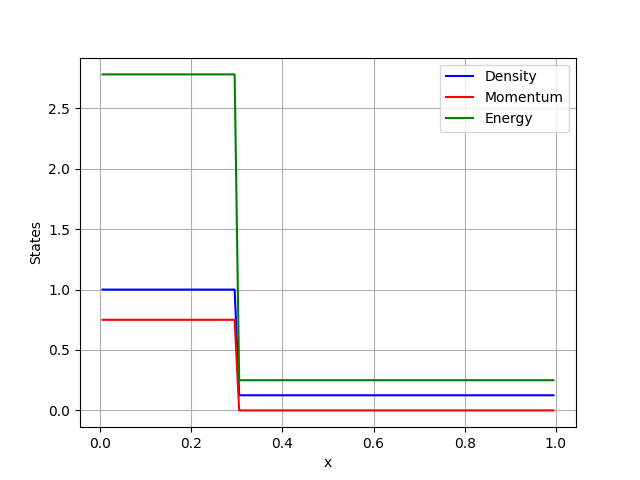
\includegraphics[width=10cm]{fig/InitialCondition.png}
    \caption{Initial condition for the modified Sod shock tube problem}
    \label{fig:ShockTubeInitialConditon}
\end{figure}
We proceed to solve the problem via a 1D finite volume solver utilizing the Roe flux.

\subsubsection{Results}
\begin{figure}[H]
    \centering
    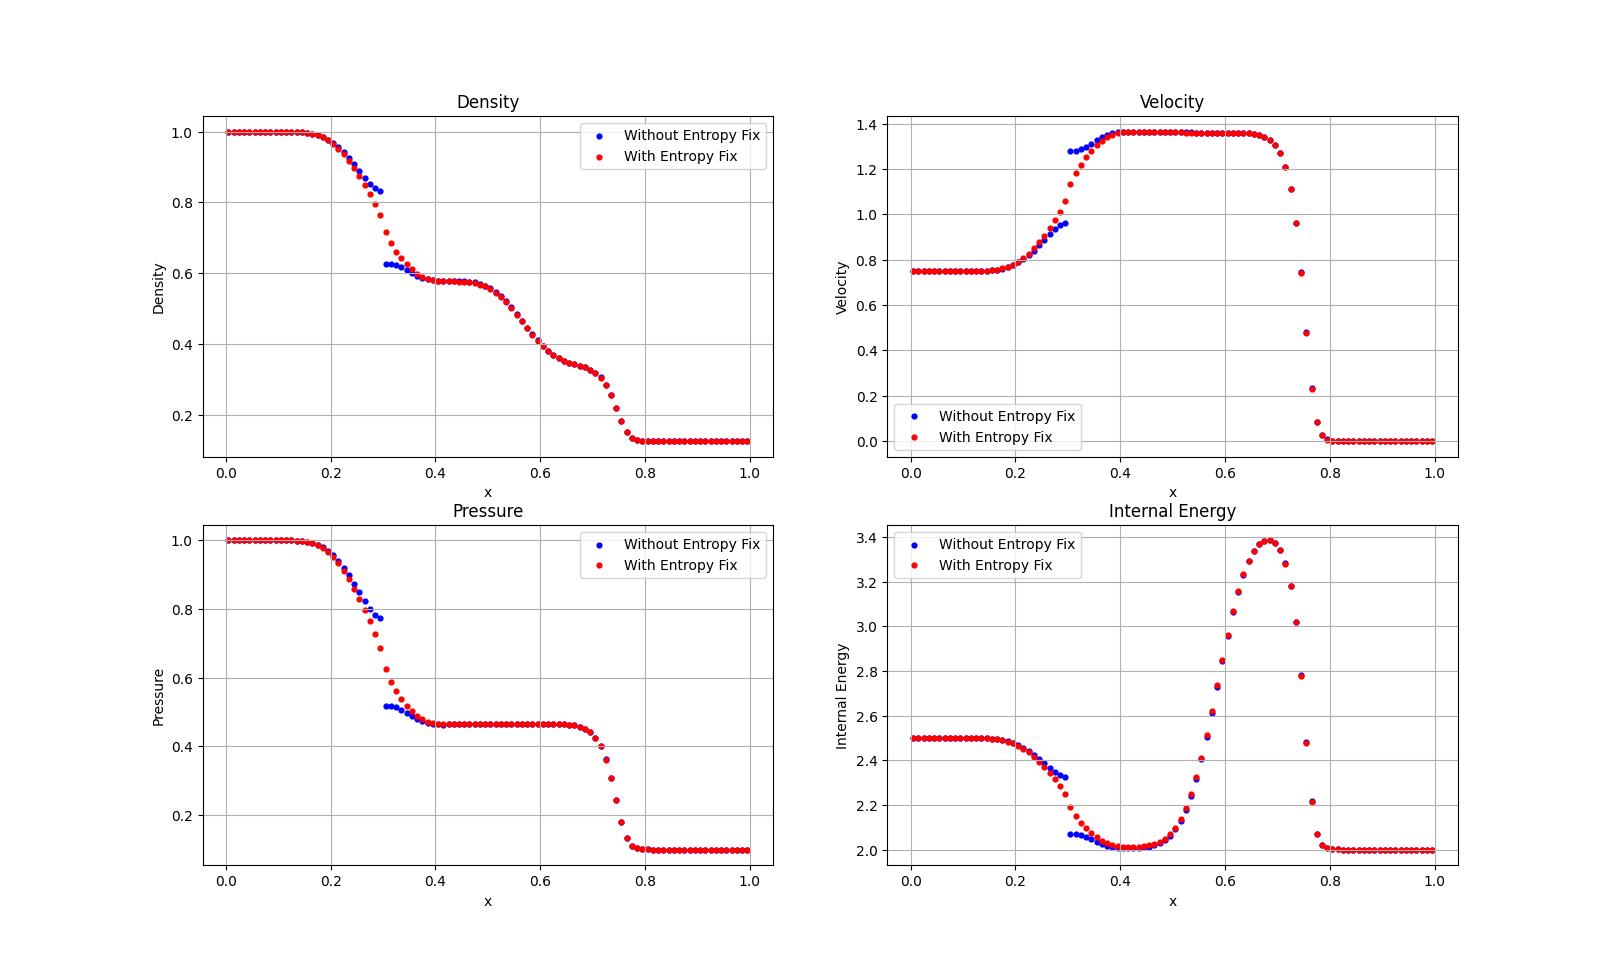
\includegraphics[width=17cm]{fig/Sod_shock_tube_results.png}
    \caption{Results for of the shock tube problem}
    \label{fig:ShockTubeResults}
\end{figure}
Figure \ref{fig:ShockTubeResults} illustrates the results of the shock tube problem, both with and without the entropy fix. We could clearly observe that without the entropy fix, there exists an unphysical discontinuity located within the sonic rarefraction $x_0 \approx 0.3$. With the entropy fix, however, the plot becomes continous and the solution appears much more physical. 

We again recall Tadmor's entropy criterion in terms of Euler's equation introduced by Roe:
\begin{equation} \label{eq:TadmorCriterion}
    \big[\mathbf{v}\big] \cdot f^*_{\text{new}} \leq \big[\rho u\big]
\end{equation}
where:
\begin{equation}
    \begin{split}
        \mathbf{v} &= 
        \begin{pmatrix}
            \frac{\gamma - S}{\gamma - 1}-\frac{\rho u^2}{2p} \\
            \frac{m}{p}\\
            -\frac{\rho}{p}
        \end{pmatrix}\\
        \Psi &= \rho u
    \end{split}
\end{equation} 
We could physically calculate the above quantities and assess whether the Roe flux is \textit{entropy conservative}. We obtain the following plot (Figure \ref{fig:TadmorResults}).
\begin{figure}[H]
    \centering
    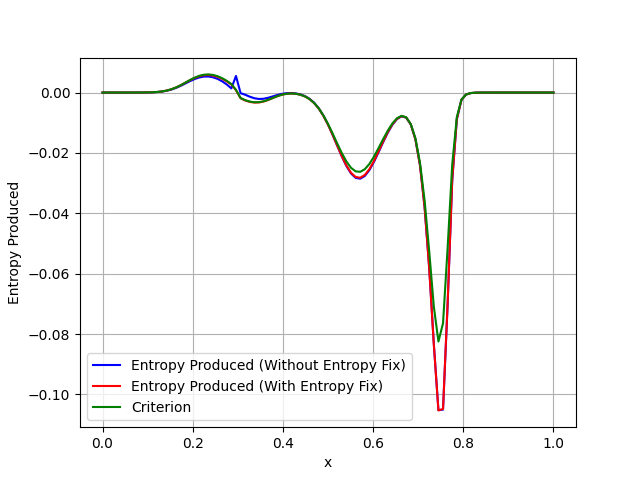
\includegraphics[width=13cm]{fig/Tadmor_Criterion.png}
    \caption{Entropy production based on Tadmor's conservative criteria}
    \label{fig:TadmorResults}
\end{figure}
We see that \textit{without} the entropy fix, there exists a sharp peak that overshoots the entropy conservative criterion at the location of the sonic rarefraction $x \approx 0.3$. This then contributed to the unphysical states predicted by the original Roe flux. With the entropy fix, however, the entropy produced by the new Roe flux exactly matches that of the criterion, illustrating that the entropy-fixed Roe flux is entropy conservative at sonic rarefractions. This is also analogous to the idea in gas dynamics, where expansion fans are \textit{isentropic} and entropy is \textit{conserved} across the process. 

Speaking of entropy production, it is interesting to look at behavior across contact discontinuity and shock ($x \approx 0.55$ and $x \approx 0.75$). Across both discontinuities, the entropy is not preserved but \textit{decreased}. In terms of Tadmor's criterion, this trend satisfies the inequality given by Equation \ref{eq:TadmorCriterion}. From a thermodynamic point of view, this result also makes sense as entropy is not conserved across shock but is \textit{increased}. In the mathematical definition of entropy, the direction that maintains a physical solution is of \textit{decreasing} entropy, which is what we observe here for the entropy-fixed Roe flux. Therefore, through a numerical experiment, we have proven that the entropy-fixed Roe flux is indeed entropy stable.

%---------------------------------------------------------------------------------------------
\bibliographystyle{plain} % We choose the "plain" reference style
\bibliography{refs} % Entries are in the refs.bib file

\end{document}